% Options for packages loaded elsewhere
\PassOptionsToPackage{unicode}{hyperref}
\PassOptionsToPackage{hyphens}{url}
\PassOptionsToPackage{dvipsnames,svgnames,x11names}{xcolor}
%
\documentclass[
  letterpaper,
  DIV=11,
  numbers=noendperiod]{scrartcl}

\usepackage{amsmath,amssymb}
\usepackage{iftex}
\ifPDFTeX
  \usepackage[T1]{fontenc}
  \usepackage[utf8]{inputenc}
  \usepackage{textcomp} % provide euro and other symbols
\else % if luatex or xetex
  \usepackage{unicode-math}
  \defaultfontfeatures{Scale=MatchLowercase}
  \defaultfontfeatures[\rmfamily]{Ligatures=TeX,Scale=1}
\fi
\usepackage{lmodern}
\ifPDFTeX\else  
    % xetex/luatex font selection
\fi
% Use upquote if available, for straight quotes in verbatim environments
\IfFileExists{upquote.sty}{\usepackage{upquote}}{}
\IfFileExists{microtype.sty}{% use microtype if available
  \usepackage[]{microtype}
  \UseMicrotypeSet[protrusion]{basicmath} % disable protrusion for tt fonts
}{}
\makeatletter
\@ifundefined{KOMAClassName}{% if non-KOMA class
  \IfFileExists{parskip.sty}{%
    \usepackage{parskip}
  }{% else
    \setlength{\parindent}{0pt}
    \setlength{\parskip}{6pt plus 2pt minus 1pt}}
}{% if KOMA class
  \KOMAoptions{parskip=half}}
\makeatother
\usepackage{xcolor}
\setlength{\emergencystretch}{3em} % prevent overfull lines
\setcounter{secnumdepth}{-\maxdimen} % remove section numbering
% Make \paragraph and \subparagraph free-standing
\makeatletter
\ifx\paragraph\undefined\else
  \let\oldparagraph\paragraph
  \renewcommand{\paragraph}{
    \@ifstar
      \xxxParagraphStar
      \xxxParagraphNoStar
  }
  \newcommand{\xxxParagraphStar}[1]{\oldparagraph*{#1}\mbox{}}
  \newcommand{\xxxParagraphNoStar}[1]{\oldparagraph{#1}\mbox{}}
\fi
\ifx\subparagraph\undefined\else
  \let\oldsubparagraph\subparagraph
  \renewcommand{\subparagraph}{
    \@ifstar
      \xxxSubParagraphStar
      \xxxSubParagraphNoStar
  }
  \newcommand{\xxxSubParagraphStar}[1]{\oldsubparagraph*{#1}\mbox{}}
  \newcommand{\xxxSubParagraphNoStar}[1]{\oldsubparagraph{#1}\mbox{}}
\fi
\makeatother

\usepackage{color}
\usepackage{fancyvrb}
\newcommand{\VerbBar}{|}
\newcommand{\VERB}{\Verb[commandchars=\\\{\}]}
\DefineVerbatimEnvironment{Highlighting}{Verbatim}{commandchars=\\\{\}}
% Add ',fontsize=\small' for more characters per line
\usepackage{framed}
\definecolor{shadecolor}{RGB}{241,243,245}
\newenvironment{Shaded}{\begin{snugshade}}{\end{snugshade}}
\newcommand{\AlertTok}[1]{\textcolor[rgb]{0.68,0.00,0.00}{#1}}
\newcommand{\AnnotationTok}[1]{\textcolor[rgb]{0.37,0.37,0.37}{#1}}
\newcommand{\AttributeTok}[1]{\textcolor[rgb]{0.40,0.45,0.13}{#1}}
\newcommand{\BaseNTok}[1]{\textcolor[rgb]{0.68,0.00,0.00}{#1}}
\newcommand{\BuiltInTok}[1]{\textcolor[rgb]{0.00,0.23,0.31}{#1}}
\newcommand{\CharTok}[1]{\textcolor[rgb]{0.13,0.47,0.30}{#1}}
\newcommand{\CommentTok}[1]{\textcolor[rgb]{0.37,0.37,0.37}{#1}}
\newcommand{\CommentVarTok}[1]{\textcolor[rgb]{0.37,0.37,0.37}{\textit{#1}}}
\newcommand{\ConstantTok}[1]{\textcolor[rgb]{0.56,0.35,0.01}{#1}}
\newcommand{\ControlFlowTok}[1]{\textcolor[rgb]{0.00,0.23,0.31}{\textbf{#1}}}
\newcommand{\DataTypeTok}[1]{\textcolor[rgb]{0.68,0.00,0.00}{#1}}
\newcommand{\DecValTok}[1]{\textcolor[rgb]{0.68,0.00,0.00}{#1}}
\newcommand{\DocumentationTok}[1]{\textcolor[rgb]{0.37,0.37,0.37}{\textit{#1}}}
\newcommand{\ErrorTok}[1]{\textcolor[rgb]{0.68,0.00,0.00}{#1}}
\newcommand{\ExtensionTok}[1]{\textcolor[rgb]{0.00,0.23,0.31}{#1}}
\newcommand{\FloatTok}[1]{\textcolor[rgb]{0.68,0.00,0.00}{#1}}
\newcommand{\FunctionTok}[1]{\textcolor[rgb]{0.28,0.35,0.67}{#1}}
\newcommand{\ImportTok}[1]{\textcolor[rgb]{0.00,0.46,0.62}{#1}}
\newcommand{\InformationTok}[1]{\textcolor[rgb]{0.37,0.37,0.37}{#1}}
\newcommand{\KeywordTok}[1]{\textcolor[rgb]{0.00,0.23,0.31}{\textbf{#1}}}
\newcommand{\NormalTok}[1]{\textcolor[rgb]{0.00,0.23,0.31}{#1}}
\newcommand{\OperatorTok}[1]{\textcolor[rgb]{0.37,0.37,0.37}{#1}}
\newcommand{\OtherTok}[1]{\textcolor[rgb]{0.00,0.23,0.31}{#1}}
\newcommand{\PreprocessorTok}[1]{\textcolor[rgb]{0.68,0.00,0.00}{#1}}
\newcommand{\RegionMarkerTok}[1]{\textcolor[rgb]{0.00,0.23,0.31}{#1}}
\newcommand{\SpecialCharTok}[1]{\textcolor[rgb]{0.37,0.37,0.37}{#1}}
\newcommand{\SpecialStringTok}[1]{\textcolor[rgb]{0.13,0.47,0.30}{#1}}
\newcommand{\StringTok}[1]{\textcolor[rgb]{0.13,0.47,0.30}{#1}}
\newcommand{\VariableTok}[1]{\textcolor[rgb]{0.07,0.07,0.07}{#1}}
\newcommand{\VerbatimStringTok}[1]{\textcolor[rgb]{0.13,0.47,0.30}{#1}}
\newcommand{\WarningTok}[1]{\textcolor[rgb]{0.37,0.37,0.37}{\textit{#1}}}

\providecommand{\tightlist}{%
  \setlength{\itemsep}{0pt}\setlength{\parskip}{0pt}}\usepackage{longtable,booktabs,array}
\usepackage{calc} % for calculating minipage widths
% Correct order of tables after \paragraph or \subparagraph
\usepackage{etoolbox}
\makeatletter
\patchcmd\longtable{\par}{\if@noskipsec\mbox{}\fi\par}{}{}
\makeatother
% Allow footnotes in longtable head/foot
\IfFileExists{footnotehyper.sty}{\usepackage{footnotehyper}}{\usepackage{footnote}}
\makesavenoteenv{longtable}
\usepackage{graphicx}
\makeatletter
\newsavebox\pandoc@box
\newcommand*\pandocbounded[1]{% scales image to fit in text height/width
  \sbox\pandoc@box{#1}%
  \Gscale@div\@tempa{\textheight}{\dimexpr\ht\pandoc@box+\dp\pandoc@box\relax}%
  \Gscale@div\@tempb{\linewidth}{\wd\pandoc@box}%
  \ifdim\@tempb\p@<\@tempa\p@\let\@tempa\@tempb\fi% select the smaller of both
  \ifdim\@tempa\p@<\p@\scalebox{\@tempa}{\usebox\pandoc@box}%
  \else\usebox{\pandoc@box}%
  \fi%
}
% Set default figure placement to htbp
\def\fps@figure{htbp}
\makeatother

\usepackage{booktabs}
\usepackage{longtable}
\usepackage{array}
\usepackage{multirow}
\usepackage{wrapfig}
\usepackage{float}
\usepackage{colortbl}
\usepackage{pdflscape}
\usepackage{tabu}
\usepackage{threeparttable}
\usepackage{threeparttablex}
\usepackage[normalem]{ulem}
\usepackage{makecell}
\usepackage{xcolor}
\KOMAoption{captions}{tableheading}
\makeatletter
\@ifpackageloaded{caption}{}{\usepackage{caption}}
\AtBeginDocument{%
\ifdefined\contentsname
  \renewcommand*\contentsname{Table of contents}
\else
  \newcommand\contentsname{Table of contents}
\fi
\ifdefined\listfigurename
  \renewcommand*\listfigurename{List of Figures}
\else
  \newcommand\listfigurename{List of Figures}
\fi
\ifdefined\listtablename
  \renewcommand*\listtablename{List of Tables}
\else
  \newcommand\listtablename{List of Tables}
\fi
\ifdefined\figurename
  \renewcommand*\figurename{Figure}
\else
  \newcommand\figurename{Figure}
\fi
\ifdefined\tablename
  \renewcommand*\tablename{Table}
\else
  \newcommand\tablename{Table}
\fi
}
\@ifpackageloaded{float}{}{\usepackage{float}}
\floatstyle{ruled}
\@ifundefined{c@chapter}{\newfloat{codelisting}{h}{lop}}{\newfloat{codelisting}{h}{lop}[chapter]}
\floatname{codelisting}{Listing}
\newcommand*\listoflistings{\listof{codelisting}{List of Listings}}
\makeatother
\makeatletter
\makeatother
\makeatletter
\@ifpackageloaded{caption}{}{\usepackage{caption}}
\@ifpackageloaded{subcaption}{}{\usepackage{subcaption}}
\makeatother

\usepackage{bookmark}

\IfFileExists{xurl.sty}{\usepackage{xurl}}{} % add URL line breaks if available
\urlstyle{same} % disable monospaced font for URLs
\hypersetup{
  pdftitle={MOCA/DAWA cluster randomized trial},
  pdfauthor={A.Amstutz},
  colorlinks=true,
  linkcolor={blue},
  filecolor={Maroon},
  citecolor={Blue},
  urlcolor={Blue},
  pdfcreator={LaTeX via pandoc}}


\title{MOCA/DAWA cluster randomized trial}
\author{A.Amstutz}
\date{}

\begin{document}
\maketitle

\renewcommand*\contentsname{Table of contents}
{
\hypersetup{linkcolor=}
\setcounter{tocdepth}{3}
\tableofcontents
}

\section{DAWA cluster randomized trial
(CRT)}\label{dawa-cluster-randomized-trial-crt}

Interventions on the level of health care workers to reduce antibiotic
prescriptions at health facilities in Zanzibar. Multi-arm with 2
interventions:

\begin{itemize}
\item
  \textbf{Control}: Standard of care
\item
  \textbf{Intervention 1}: eHealth tool (CDSS \& nudging)
\item
  \textbf{Intervention 2}: eHealth tool (CDSS \& nudging) + AMR
  stewardship clubs
\end{itemize}

\subsection{Parameters}\label{parameters}

\begin{itemize}
\item
  Eligible participants: Patients attending the dispensary with acute
  infectious illness
\item
  Power for subgroup of kids under 5 years (special subgroup of
  interest), ca. 33\% of all attending patients
\item
  Cluster size of eligible overall participants: 80-500 per cluster per
  month (cluster size variation!)
\item
  Cluster size of eligible kids under 5 years: 26-165 per cluster per
  month
\item
  Max. 39 clusters (health dispensaries) due to feasibility/budget
\item
  Binary outcome: Proportion of patients prescribed an antibiotic at
  first presentation to care
\item
  Baseline prescription rate in control clusters: 75\%, based on data
  from existing facilities but some variability
\item
  Expected delta Control to Intervention 1: 25 percentage points, based
  on previous studies in same setting
\item
  Expected delta Control to Intervention 2: 30 percentage points
\item
  Intervention 1 vs Intervention 2 not of primary interest
\item
  Desired power min. 80\%
\item
  ICC for AB prescription: 0.2, based on previous studies in same
  setting, but some uncertainty
\item
  Mean cluster size: 40/month, but high variability (ratio of standard
  deviation of cluster sizes to mean of cluster sizes: 0.5-0.6)
\item
  We expect intervention effect to manifest 3-4 months after baseline
\item
  Important feasibility aspect: The primary outcome is collected through
  routine data, while the key secondary outcomes are collected via phone
  calls
\end{itemize}

\subsection{Design considerations}\label{design-considerations}

\begin{itemize}
\tightlist
\item
  3-arm vs 2x 2-arm? -\textgreater{} final decision: 3-arm
\end{itemize}

\begin{itemize}
\item
  Recruitment bias? -\textgreater{} see protocol how to mitigate
\item
  Secular trend? -\textgreater{} see protocol re secondary outcome
\item
  Which pair-wise comparisons to power for? -\textgreater{} the smaller
  delta comparison
\item
  Multiplicity? -\textgreater{} see separate discussion; decision: No
  adjustment for multiplicity
\end{itemize}

\textbf{Packages}

\begin{Shaded}
\begin{Highlighting}[]
\FunctionTok{RNGkind}\NormalTok{(}\StringTok{"L\textquotesingle{}Ecuyer{-}CMRG"}\NormalTok{) }\CommentTok{\# simstudy}
\FunctionTok{set.seed}\NormalTok{(}\DecValTok{19287}\NormalTok{) }\CommentTok{\# for reproducibility}
\FunctionTok{library}\NormalTok{(simstudy)}
\FunctionTok{library}\NormalTok{(parallel) }\CommentTok{\# for parallelization of core (max 8 on my laptop)}

\FunctionTok{library}\NormalTok{(lme4)}
\FunctionTok{library}\NormalTok{(marginaleffects) }\CommentTok{\# marginal standardization}
\FunctionTok{library}\NormalTok{(insight) }\CommentTok{\# robust SE}
\FunctionTok{library}\NormalTok{(geepack) }\CommentTok{\# to tackle alternative and more robust (but less efficient?) estimands}

\FunctionTok{library}\NormalTok{(dplyr)}
\FunctionTok{library}\NormalTok{(pwr)}
\FunctionTok{library}\NormalTok{(ggplot2)}
\FunctionTok{library}\NormalTok{(kableExtra)}
\end{Highlighting}
\end{Shaded}

\section{Corresponding individual randomized
trial}\label{corresponding-individual-randomized-trial}

Sample size for the individual randomized trial on the same question

\begin{Shaded}
\begin{Highlighting}[]
\CommentTok{\# Parameters}
\NormalTok{p\_C }\OtherTok{\textless{}{-}} \FloatTok{0.75} \CommentTok{\# control: Baseline prescription rate}
\NormalTok{p\_I1 }\OtherTok{\textless{}{-}} \FloatTok{0.50} \CommentTok{\# int 1: 25pp reduction}
\NormalTok{p\_I2 }\OtherTok{\textless{}{-}} \FloatTok{0.50} \CommentTok{\# int 2: 30pp reduction}
\NormalTok{power }\OtherTok{\textless{}{-}} \FloatTok{0.80} \CommentTok{\# desired power}
\NormalTok{alpha }\OtherTok{\textless{}{-}} \FloatTok{0.05} \CommentTok{\# do not apply any (bonferroni) correction for multiplicity (see separate discussion)}

\CommentTok{\# Effect sizes}
\NormalTok{h\_I1\_C }\OtherTok{\textless{}{-}} \FunctionTok{ES.h}\NormalTok{(}\AttributeTok{p1 =}\NormalTok{ p\_I1, }\AttributeTok{p2 =}\NormalTok{ p\_C)}
\NormalTok{h\_I2\_C }\OtherTok{\textless{}{-}} \FunctionTok{ES.h}\NormalTok{(}\AttributeTok{p1 =}\NormalTok{ p\_I2, }\AttributeTok{p2 =}\NormalTok{ p\_C)}

\FunctionTok{cat}\NormalTok{(}\StringTok{"Cohen\textquotesingle{}s h for I1 vs Control:"}\NormalTok{, }\FunctionTok{round}\NormalTok{(h\_I1\_C, }\DecValTok{3}\NormalTok{), }\StringTok{"}\SpecialCharTok{\textbackslash{}n}\StringTok{"}\NormalTok{)}
\end{Highlighting}
\end{Shaded}

\begin{verbatim}
Cohen's h for I1 vs Control: -0.524 
\end{verbatim}

\begin{Shaded}
\begin{Highlighting}[]
\FunctionTok{cat}\NormalTok{(}\StringTok{"Cohen\textquotesingle{}s h for I2 vs Control:"}\NormalTok{, }\FunctionTok{round}\NormalTok{(h\_I2\_C, }\DecValTok{3}\NormalTok{), }\StringTok{"}\SpecialCharTok{\textbackslash{}n}\StringTok{"}\NormalTok{)}
\end{Highlighting}
\end{Shaded}

\begin{verbatim}
Cohen's h for I2 vs Control: -0.524 
\end{verbatim}

\begin{Shaded}
\begin{Highlighting}[]
\CommentTok{\# =\textgreater{} reduction of mind. 25\% is a Cohen\textquotesingle{}s h of over 0.5 {-}\textgreater{} medium to large effect according to Cohen}

\CommentTok{\# Sample size first pair{-}wise comparison (I1 vs C)}
\NormalTok{ss\_I1\_C }\OtherTok{\textless{}{-}} \FunctionTok{pwr.2p.test}\NormalTok{(}\AttributeTok{h =}\NormalTok{ h\_I1\_C, }\AttributeTok{sig.level =}\NormalTok{ alpha, }\AttributeTok{power =}\NormalTok{ power)}
\FunctionTok{cat}\NormalTok{(}\StringTok{"Sample size per arm (I1 vs C):"}\NormalTok{, }\FunctionTok{ceiling}\NormalTok{(ss\_I1\_C}\SpecialCharTok{$}\NormalTok{n), }\StringTok{"}\SpecialCharTok{\textbackslash{}n}\StringTok{"}\NormalTok{)}
\end{Highlighting}
\end{Shaded}

\begin{verbatim}
Sample size per arm (I1 vs C): 58 
\end{verbatim}

\begin{Shaded}
\begin{Highlighting}[]
\CommentTok{\# Sample size second pair{-}wise comparison (I2 vs C)}
\NormalTok{ss\_I2\_C }\OtherTok{\textless{}{-}} \FunctionTok{pwr.2p.test}\NormalTok{(}\AttributeTok{h =}\NormalTok{ h\_I2\_C, }\AttributeTok{sig.level =}\NormalTok{ alpha, }\AttributeTok{power =}\NormalTok{ power)}
\FunctionTok{cat}\NormalTok{(}\StringTok{"Sample size per arm (I2 vs C):"}\NormalTok{, }\FunctionTok{ceiling}\NormalTok{(ss\_I2\_C}\SpecialCharTok{$}\NormalTok{n), }\StringTok{"}\SpecialCharTok{\textbackslash{}n}\StringTok{"}\NormalTok{)}
\end{Highlighting}
\end{Shaded}

\begin{verbatim}
Sample size per arm (I2 vs C): 58 
\end{verbatim}

\begin{Shaded}
\begin{Highlighting}[]
\CommentTok{\# Use max of the two}
\NormalTok{n\_per\_arm }\OtherTok{\textless{}{-}} \FunctionTok{max}\NormalTok{(}\FunctionTok{ceiling}\NormalTok{(ss\_I1\_C}\SpecialCharTok{$}\NormalTok{n), }\FunctionTok{ceiling}\NormalTok{(ss\_I2\_C}\SpecialCharTok{$}\NormalTok{n))}
\NormalTok{n\_total }\OtherTok{\textless{}{-}}\NormalTok{ n\_per\_arm }\SpecialCharTok{*} \DecValTok{3}

\FunctionTok{cat}\NormalTok{(}\StringTok{"Sample size per arm:"}\NormalTok{, n\_per\_arm, }\StringTok{"}\SpecialCharTok{\textbackslash{}n}\StringTok{"}\NormalTok{)}
\end{Highlighting}
\end{Shaded}

\begin{verbatim}
Sample size per arm: 58 
\end{verbatim}

\begin{Shaded}
\begin{Highlighting}[]
\FunctionTok{cat}\NormalTok{(}\StringTok{"Total sample size (3{-}arm trial):"}\NormalTok{, n\_total)}
\end{Highlighting}
\end{Shaded}

\begin{verbatim}
Total sample size (3-arm trial): 174
\end{verbatim}

A reduction of at least 25\% percentage points (the smaller delta of the
two) represents a Cohen's h of \textgreater0.5 =\textgreater{} medium to
large effect

\section{Now, move to a CRT design}\label{now-move-to-a-crt-design}

\subsection{\texorpdfstring{\textbf{(1) Standard sample size
calculation}}{(1) Standard sample size calculation}}\label{standard-sample-size-calculation}

\textbf{Figure out the design effect (DEFF) for clustering, to add to
the individual RCT sample size}

The usual standard DEFF formula:

DEFF = 1+(m−1)*ICC , whereby m = cluster size

However, let's not forget the cluster size variation! The usual
conservative adjustment of the DEFF with cluster size variation is:

DEFF\_cv = 1+((m\emph{(1+CV\^{}2)−1))}ICC , whereby CV is the
coefficient of variation (ratio of standard deviation of cluster sizes
to mean of cluster sizes)

See here:
\hyperref[0]{https://pmc.ncbi.nlm.nih.gov/articles/PMC7394950/\#sup1}

Since, we have flexibility in individual sample size per cluster and
need to restrict it anyway to keep the data collection for the key
secondary outcomes feasible, we decided to take a random sample, same n,
from each cluster =\textgreater{} CV = 0. And we stratify the
randomization and adjust the outcome model for actual cluster size
(attendance rate)

An individual sample size per cluster (i.e.~mean cluster size) of n=150
will be feasible to recruit during 2 months (month 4 and 5 after
baseline) from each cluster, using a random sampling strategy. That
means we will get n=40 per cluster for our subgroup interest (kids under
5) with minimal CV (CV=0.1).

\begin{Shaded}
\begin{Highlighting}[]
\CommentTok{\# Parameters}
\NormalTok{p\_C }\OtherTok{\textless{}{-}} \FloatTok{0.75} \CommentTok{\# control: Baseline prescription rate}
\NormalTok{p\_I1 }\OtherTok{\textless{}{-}} \FloatTok{0.50} \CommentTok{\# int 1: 25pp reduction}
\NormalTok{p\_I2 }\OtherTok{\textless{}{-}} \FloatTok{0.45} \CommentTok{\# int 2: 30pp reduction}
\NormalTok{power }\OtherTok{\textless{}{-}} \FloatTok{0.80} \CommentTok{\# desired power}
\NormalTok{ICC }\OtherTok{\textless{}{-}} \FloatTok{0.20}
\NormalTok{alpha }\OtherTok{\textless{}{-}} \FloatTok{0.05} \CommentTok{\# do not apply any (bonferroni) correction for multiplicity (see separate discussion). Bonferroni would be alpha\_familywise / number of comparisons (=2)}

\NormalTok{m }\OtherTok{\textless{}{-}} \DecValTok{40}
\NormalTok{CV }\OtherTok{\textless{}{-}} \FloatTok{0.1} \CommentTok{\# 0 = no cluster size variation}

\NormalTok{deff }\OtherTok{\textless{}{-}} \DecValTok{1}\SpecialCharTok{+}\NormalTok{(m}\DecValTok{{-}1}\NormalTok{)}\SpecialCharTok{*}\NormalTok{ICC }\CommentTok{\# standard DEFF}
\NormalTok{deff\_cv }\OtherTok{\textless{}{-}} \DecValTok{1}\SpecialCharTok{+}\NormalTok{((m}\SpecialCharTok{*}\NormalTok{(}\DecValTok{1}\SpecialCharTok{+}\NormalTok{CV}\SpecialCharTok{\^{}}\DecValTok{2}\NormalTok{))}\SpecialCharTok{{-}}\DecValTok{1}\NormalTok{)}\SpecialCharTok{*}\NormalTok{ICC }\CommentTok{\# DEFF with cluster size variation}

\CommentTok{\# Effect sizes}
\NormalTok{h\_I1\_C }\OtherTok{\textless{}{-}} \FunctionTok{ES.h}\NormalTok{(}\AttributeTok{p1 =}\NormalTok{ p\_I1, }\AttributeTok{p2 =}\NormalTok{ p\_C)}
\NormalTok{h\_I2\_C }\OtherTok{\textless{}{-}} \FunctionTok{ES.h}\NormalTok{(}\AttributeTok{p1 =}\NormalTok{ p\_I2, }\AttributeTok{p2 =}\NormalTok{ p\_C)}

\CommentTok{\# Individual RCT sample sizes for both contrasts}
\NormalTok{ss1 }\OtherTok{\textless{}{-}} \FunctionTok{pwr.2p.test}\NormalTok{(}\AttributeTok{h =}\NormalTok{ h\_I1\_C, }\AttributeTok{power =} \FloatTok{0.80}\NormalTok{, }\AttributeTok{sig.level =}\NormalTok{ alpha)}\SpecialCharTok{$}\NormalTok{n}
\NormalTok{ss2 }\OtherTok{\textless{}{-}} \FunctionTok{pwr.2p.test}\NormalTok{(}\AttributeTok{h =}\NormalTok{ h\_I2\_C, }\AttributeTok{power =} \FloatTok{0.80}\NormalTok{, }\AttributeTok{sig.level =}\NormalTok{ alpha)}\SpecialCharTok{$}\NormalTok{n}

\CommentTok{\# CRT sample sizes for both contrasts}
\NormalTok{ss1\_crt }\OtherTok{\textless{}{-}} \FunctionTok{ceiling}\NormalTok{(ss1 }\SpecialCharTok{*}\NormalTok{ deff\_cv)}
\NormalTok{ss2\_crt }\OtherTok{\textless{}{-}} \FunctionTok{ceiling}\NormalTok{(ss2 }\SpecialCharTok{*}\NormalTok{ deff\_cv)}

\CommentTok{\# Contrast 1 (smaller Delta/Cohens\textquotesingle{}d =\textgreater{} determines overall cluster number)}
\NormalTok{n\_clusters1 }\OtherTok{\textless{}{-}} \FunctionTok{ceiling}\NormalTok{(ss1\_crt }\SpecialCharTok{/}\NormalTok{ m)}
\FunctionTok{cat}\NormalTok{(}\StringTok{"Cluster sample size int arm 1:"}\NormalTok{, n\_clusters1, }\StringTok{"}\SpecialCharTok{\textbackslash{}n}\StringTok{"}\NormalTok{)}
\end{Highlighting}
\end{Shaded}

\begin{verbatim}
Cluster sample size int arm 1: 13 
\end{verbatim}

\begin{Shaded}
\begin{Highlighting}[]
\FunctionTok{cat}\NormalTok{(}\StringTok{"Individual sample size int arm 1:"}\NormalTok{, ss1\_crt, }\StringTok{"}\SpecialCharTok{\textbackslash{}n}\StringTok{"}\NormalTok{)}
\end{Highlighting}
\end{Shaded}

\begin{verbatim}
Individual sample size int arm 1: 509 
\end{verbatim}

\begin{Shaded}
\begin{Highlighting}[]
\CommentTok{\# Contrast 2}
\NormalTok{n\_clusters2 }\OtherTok{\textless{}{-}} \FunctionTok{ceiling}\NormalTok{(ss2\_crt }\SpecialCharTok{/}\NormalTok{ m)}
\FunctionTok{cat}\NormalTok{(}\StringTok{"Cluster sample size int arm 2:"}\NormalTok{, n\_clusters2, }\StringTok{"}\SpecialCharTok{\textbackslash{}n}\StringTok{"}\NormalTok{)}
\end{Highlighting}
\end{Shaded}

\begin{verbatim}
Cluster sample size int arm 2: 9 
\end{verbatim}

\begin{Shaded}
\begin{Highlighting}[]
\FunctionTok{cat}\NormalTok{(}\StringTok{"Individual sample size int arm 2:"}\NormalTok{, ss2\_crt, }\StringTok{"}\SpecialCharTok{\textbackslash{}n}\StringTok{"}\NormalTok{)}
\end{Highlighting}
\end{Shaded}

\begin{verbatim}
Individual sample size int arm 2: 359 
\end{verbatim}

\begin{Shaded}
\begin{Highlighting}[]
\CommentTok{\# Total}
\NormalTok{tot\_clusters }\OtherTok{\textless{}{-}}\NormalTok{ n\_clusters1 }\SpecialCharTok{*} \DecValTok{3}
\NormalTok{tot\_ind }\OtherTok{\textless{}{-}}\NormalTok{ ss1\_crt }\SpecialCharTok{*} \DecValTok{3}
\FunctionTok{cat}\NormalTok{(}\StringTok{"Total cluster sample size:"}\NormalTok{, tot\_clusters, }\StringTok{"}\SpecialCharTok{\textbackslash{}n}\StringTok{"}\NormalTok{)}
\end{Highlighting}
\end{Shaded}

\begin{verbatim}
Total cluster sample size: 39 
\end{verbatim}

\begin{Shaded}
\begin{Highlighting}[]
\FunctionTok{cat}\NormalTok{(}\StringTok{"Total individual sample size:"}\NormalTok{, tot\_ind, }\StringTok{"}\SpecialCharTok{\textbackslash{}n}\StringTok{"}\NormalTok{)}
\end{Highlighting}
\end{Shaded}

\begin{verbatim}
Total individual sample size: 1527 
\end{verbatim}

\subsubsection{\texorpdfstring{\textbf{(1.1) Varying assumptions -
Standard sample size
calculation}}{(1.1) Varying assumptions - Standard sample size calculation}}\label{varying-assumptions---standard-sample-size-calculation}

\paragraph{\texorpdfstring{\textbf{(1.1.1) Varying baseline control
rate}}{(1.1.1) Varying baseline control rate}}\label{varying-baseline-control-rate}

All parameters fixed, except baseline control rate versus number of
clusters \& individuals needed

\begin{Shaded}
\begin{Highlighting}[]
\CommentTok{\# Define fixed parameters}
\NormalTok{power }\OtherTok{\textless{}{-}} \FloatTok{0.80}
\NormalTok{alpha }\OtherTok{\textless{}{-}} \FloatTok{0.05}
\NormalTok{ICC }\OtherTok{\textless{}{-}} \FloatTok{0.20}
\NormalTok{CV }\OtherTok{\textless{}{-}} \FloatTok{0.1}
\NormalTok{m }\OtherTok{\textless{}{-}} \DecValTok{40}

\CommentTok{\# Baseline control rates to test}
\NormalTok{p\_C\_values }\OtherTok{\textless{}{-}} \FunctionTok{seq}\NormalTok{(}\FloatTok{0.60}\NormalTok{, }\FloatTok{0.85}\NormalTok{, }\AttributeTok{by =} \FloatTok{0.05}\NormalTok{)}

\CommentTok{\# Initialize an empty dataframe to store results}
\NormalTok{results\_df }\OtherTok{\textless{}{-}} \FunctionTok{data.frame}\NormalTok{(}
  \AttributeTok{p\_C =} \FunctionTok{numeric}\NormalTok{(),}
  \AttributeTok{n\_clusters\_per\_arm =} \FunctionTok{numeric}\NormalTok{(),}
  \AttributeTok{n\_individuals\_per\_arm =} \FunctionTok{numeric}\NormalTok{()}
\NormalTok{)}

\CommentTok{\# Function to calculate Cohen\textquotesingle{}s h for two proportions}
\NormalTok{cohen\_h }\OtherTok{\textless{}{-}} \ControlFlowTok{function}\NormalTok{(p1, p2) \{}
  \DecValTok{2} \SpecialCharTok{*}\NormalTok{ (}\FunctionTok{asin}\NormalTok{(}\FunctionTok{sqrt}\NormalTok{(p1)) }\SpecialCharTok{{-}} \FunctionTok{asin}\NormalTok{(}\FunctionTok{sqrt}\NormalTok{(p2)))}
\NormalTok{\}}

\CommentTok{\# Loop through each baseline control rate}
\ControlFlowTok{for}\NormalTok{ (p\_C }\ControlFlowTok{in}\NormalTok{ p\_C\_values) \{}
  \CommentTok{\# Intervention rates based on percentage point reductions}
\NormalTok{  p\_I1 }\OtherTok{\textless{}{-}}\NormalTok{ p\_C }\SpecialCharTok{{-}} \FloatTok{0.25}
\NormalTok{  p\_I2 }\OtherTok{\textless{}{-}}\NormalTok{ p\_C }\SpecialCharTok{{-}} \FloatTok{0.30}
  
  \CommentTok{\# Skip if intervention rates are invalid (less than 0)}
  \ControlFlowTok{if}\NormalTok{ (p\_I1 }\SpecialCharTok{\textless{}} \DecValTok{0} \SpecialCharTok{|}\NormalTok{ p\_I2 }\SpecialCharTok{\textless{}} \DecValTok{0}\NormalTok{) \{}
    \ControlFlowTok{next}
\NormalTok{  \}}

  \CommentTok{\# Calculate design effect with no cluster size variation (CV = 0)}
\NormalTok{  deff\_cv }\OtherTok{\textless{}{-}} \DecValTok{1} \SpecialCharTok{+}\NormalTok{ ((m }\SpecialCharTok{*}\NormalTok{ (}\DecValTok{1} \SpecialCharTok{+}\NormalTok{ CV}\SpecialCharTok{\^{}}\DecValTok{2}\NormalTok{)) }\SpecialCharTok{{-}} \DecValTok{1}\NormalTok{) }\SpecialCharTok{*}\NormalTok{ ICC}
  
  \CommentTok{\# Effect sizes for both comparisons}
\NormalTok{  h\_I1\_C }\OtherTok{\textless{}{-}} \FunctionTok{cohen\_h}\NormalTok{(p\_I1, p\_C)}
\NormalTok{  h\_I2\_C }\OtherTok{\textless{}{-}} \FunctionTok{cohen\_h}\NormalTok{(p\_I2, p\_C)}
  
  \CommentTok{\# Individual RCT sample sizes for both contrasts}
\NormalTok{  ss1 }\OtherTok{\textless{}{-}} \FunctionTok{pwr.2p.test}\NormalTok{(}\AttributeTok{h =}\NormalTok{ h\_I1\_C, }\AttributeTok{power =}\NormalTok{ power, }\AttributeTok{sig.level =}\NormalTok{ alpha)}\SpecialCharTok{$}\NormalTok{n}
\NormalTok{  ss2 }\OtherTok{\textless{}{-}} \FunctionTok{pwr.2p.test}\NormalTok{(}\AttributeTok{h =}\NormalTok{ h\_I2\_C, }\AttributeTok{power =}\NormalTok{ power, }\AttributeTok{sig.level =}\NormalTok{ alpha)}\SpecialCharTok{$}\NormalTok{n}
  
  \CommentTok{\# Use max of the two to be conservative}
\NormalTok{  n\_per\_arm\_rct }\OtherTok{\textless{}{-}} \FunctionTok{max}\NormalTok{(ss1, ss2)}
  
  \CommentTok{\# CRT sample size per arm (individuals)}
\NormalTok{  n\_per\_arm\_crt }\OtherTok{\textless{}{-}} \FunctionTok{ceiling}\NormalTok{(n\_per\_arm\_rct }\SpecialCharTok{*}\NormalTok{ deff\_cv)}
  
  \CommentTok{\# Number of clusters per arm}
\NormalTok{  n\_clusters\_per\_arm }\OtherTok{\textless{}{-}} \FunctionTok{ceiling}\NormalTok{(n\_per\_arm\_crt }\SpecialCharTok{/}\NormalTok{ m)}
  
  \CommentTok{\# Append results to the data frame}
\NormalTok{  results\_df }\OtherTok{\textless{}{-}} \FunctionTok{rbind}\NormalTok{(results\_df, }\FunctionTok{data.frame}\NormalTok{(}
    \AttributeTok{p\_C =}\NormalTok{ p\_C,}
    \AttributeTok{n\_clusters\_per\_arm =}\NormalTok{ n\_clusters\_per\_arm,}
    \AttributeTok{n\_individuals\_per\_arm =}\NormalTok{ n\_per\_arm\_crt}
\NormalTok{  ))}
\NormalTok{\}}
\end{Highlighting}
\end{Shaded}

\begin{Shaded}
\begin{Highlighting}[]
\CommentTok{\# Plot number of clusters needed}
\FunctionTok{ggplot}\NormalTok{(results\_df, }\FunctionTok{aes}\NormalTok{(}\AttributeTok{x =}\NormalTok{ p\_C, }\AttributeTok{y =}\NormalTok{ n\_clusters\_per\_arm }\SpecialCharTok{*} \DecValTok{3}\NormalTok{)) }\SpecialCharTok{+}
  \FunctionTok{geom\_line}\NormalTok{(}\AttributeTok{color =} \StringTok{"darkgreen"}\NormalTok{, }\AttributeTok{size =} \DecValTok{1}\NormalTok{) }\SpecialCharTok{+}
  \FunctionTok{geom\_point}\NormalTok{(}\AttributeTok{color =} \StringTok{"darkgreen"}\NormalTok{, }\AttributeTok{size =} \DecValTok{2}\NormalTok{) }\SpecialCharTok{+}
  \FunctionTok{labs}\NormalTok{(}
    \AttributeTok{title =} \StringTok{"Total clusters needed vs. Baseline control rate"}\NormalTok{,}
    \AttributeTok{x =} \StringTok{"Baseline control rate"}\NormalTok{,}
    \AttributeTok{y =} \StringTok{"Total clusters needed (for 3 arms)"}
\NormalTok{  ) }\SpecialCharTok{+}
  \FunctionTok{theme\_minimal}\NormalTok{() }\SpecialCharTok{+}
  \FunctionTok{scale\_x\_continuous}\NormalTok{(}\AttributeTok{labels =}\NormalTok{ scales}\SpecialCharTok{::}\FunctionTok{percent\_format}\NormalTok{(}\AttributeTok{accuracy =} \DecValTok{1}\NormalTok{),}
                     \AttributeTok{breaks =} \FunctionTok{seq}\NormalTok{(}\FloatTok{0.50}\NormalTok{, }\FloatTok{0.85}\NormalTok{, }\AttributeTok{by =} \FloatTok{0.02}\NormalTok{)) }\SpecialCharTok{+}
  \FunctionTok{scale\_y\_continuous}\NormalTok{(}\AttributeTok{breaks =} \FunctionTok{seq}\NormalTok{(}\DecValTok{0}\NormalTok{, }\FunctionTok{max}\NormalTok{(results\_df}\SpecialCharTok{$}\NormalTok{n\_clusters\_per\_arm }\SpecialCharTok{*} \DecValTok{3}\NormalTok{), }\AttributeTok{by =} \DecValTok{1}\NormalTok{))}
\end{Highlighting}
\end{Shaded}

\begin{verbatim}
Warning: Using `size` aesthetic for lines was deprecated in ggplot2 3.4.0.
i Please use `linewidth` instead.
\end{verbatim}

\pandocbounded{\includegraphics[keepaspectratio]{MOCA-DAWA_files/figure-pdf/unnamed-chunk-5-1.pdf}}

\begin{Shaded}
\begin{Highlighting}[]
\CommentTok{\# Plot number of individuals needed}
\FunctionTok{ggplot}\NormalTok{(results\_df, }\FunctionTok{aes}\NormalTok{(}\AttributeTok{x =}\NormalTok{ p\_C, }\AttributeTok{y =}\NormalTok{ n\_individuals\_per\_arm }\SpecialCharTok{*} \DecValTok{3}\NormalTok{)) }\SpecialCharTok{+}
  \FunctionTok{geom\_line}\NormalTok{(}\AttributeTok{color =} \StringTok{"lightgreen"}\NormalTok{, }\AttributeTok{size =} \DecValTok{1}\NormalTok{) }\SpecialCharTok{+}
  \FunctionTok{geom\_point}\NormalTok{(}\AttributeTok{color =} \StringTok{"lightgreen"}\NormalTok{, }\AttributeTok{size =} \DecValTok{2}\NormalTok{) }\SpecialCharTok{+}
  \FunctionTok{labs}\NormalTok{(}
    \AttributeTok{title =} \StringTok{"Total individuals needed vs. Baseline control rate"}\NormalTok{,}
    \AttributeTok{x =} \StringTok{"Baseline control rate"}\NormalTok{,}
    \AttributeTok{y =} \StringTok{"Total individuals needed (for 3 arms)"}
\NormalTok{  ) }\SpecialCharTok{+}
  \FunctionTok{theme\_minimal}\NormalTok{() }\SpecialCharTok{+}
  \FunctionTok{scale\_x\_continuous}\NormalTok{(}\AttributeTok{labels =}\NormalTok{ scales}\SpecialCharTok{::}\FunctionTok{percent\_format}\NormalTok{(}\AttributeTok{accuracy =} \DecValTok{1}\NormalTok{),}
                     \AttributeTok{breaks =} \FunctionTok{seq}\NormalTok{(}\FloatTok{0.60}\NormalTok{, }\FloatTok{0.85}\NormalTok{, }\AttributeTok{by =} \FloatTok{0.02}\NormalTok{)) }\SpecialCharTok{+}
  \FunctionTok{scale\_y\_continuous}\NormalTok{(}\AttributeTok{breaks =} \FunctionTok{seq}\NormalTok{(}\DecValTok{0}\NormalTok{, }\FunctionTok{max}\NormalTok{(results\_df}\SpecialCharTok{$}\NormalTok{n\_individuals\_per\_arm }\SpecialCharTok{*} \DecValTok{3}\NormalTok{), }\AttributeTok{by =} \DecValTok{50}\NormalTok{))}
\end{Highlighting}
\end{Shaded}

\pandocbounded{\includegraphics[keepaspectratio]{MOCA-DAWA_files/figure-pdf/unnamed-chunk-6-1.pdf}}

\paragraph{\texorpdfstring{\textbf{(1.1.2) Varying
ICC}}{(1.1.2) Varying ICC}}\label{varying-icc}

All parameters fixed, except ICC versus number of clusters \&
individuals needed

\begin{Shaded}
\begin{Highlighting}[]
\CommentTok{\# Define parameters}
\NormalTok{power }\OtherTok{\textless{}{-}} \FloatTok{0.80}
\NormalTok{alpha }\OtherTok{\textless{}{-}} \FloatTok{0.05}
\NormalTok{p\_C }\OtherTok{\textless{}{-}} \FloatTok{0.75} 
\NormalTok{m }\OtherTok{\textless{}{-}} \DecValTok{40}
\NormalTok{CV }\OtherTok{\textless{}{-}} \FloatTok{0.1}

\CommentTok{\# Range of ICC values to test}
\NormalTok{ICC\_values }\OtherTok{\textless{}{-}} \FunctionTok{seq}\NormalTok{(}\FloatTok{0.05}\NormalTok{, }\FloatTok{0.25}\NormalTok{, }\AttributeTok{by =} \FloatTok{0.01}\NormalTok{)}

\CommentTok{\# Initialize an empty dataframe to store results}
\NormalTok{results\_df }\OtherTok{\textless{}{-}} \FunctionTok{data.frame}\NormalTok{(}
  \AttributeTok{ICC =} \FunctionTok{numeric}\NormalTok{(),}
  \AttributeTok{n\_clusters\_per\_arm =} \FunctionTok{numeric}\NormalTok{(),}
  \AttributeTok{n\_individuals\_per\_arm =} \FunctionTok{numeric}\NormalTok{()}
\NormalTok{)}

\CommentTok{\# Function to calculate Cohen\textquotesingle{}s h for two proportions}
\NormalTok{cohen\_h }\OtherTok{\textless{}{-}} \ControlFlowTok{function}\NormalTok{(p1, p2) \{}
  \DecValTok{2} \SpecialCharTok{*}\NormalTok{ (}\FunctionTok{asin}\NormalTok{(}\FunctionTok{sqrt}\NormalTok{(p1)) }\SpecialCharTok{{-}} \FunctionTok{asin}\NormalTok{(}\FunctionTok{sqrt}\NormalTok{(p2)))}
\NormalTok{\}}

\CommentTok{\# Loop through each ICC value}
\ControlFlowTok{for}\NormalTok{ (icc }\ControlFlowTok{in}\NormalTok{ ICC\_values) \{}
  \CommentTok{\# Intervention rates based on percentage point reductions}
\NormalTok{  p\_I1 }\OtherTok{\textless{}{-}}\NormalTok{ p\_C }\SpecialCharTok{{-}} \FloatTok{0.25}
\NormalTok{  p\_I2 }\OtherTok{\textless{}{-}}\NormalTok{ p\_C }\SpecialCharTok{{-}} \FloatTok{0.30}
  
  \CommentTok{\# Calculate design effect}
\NormalTok{  deff }\OtherTok{\textless{}{-}} \DecValTok{1} \SpecialCharTok{+}\NormalTok{ (m }\SpecialCharTok{{-}} \DecValTok{1}\NormalTok{) }\SpecialCharTok{*}\NormalTok{ icc}
  
  \CommentTok{\# Effect sizes for both comparisons}
\NormalTok{  h\_I1\_C }\OtherTok{\textless{}{-}} \FunctionTok{cohen\_h}\NormalTok{(p\_I1, p\_C)}
\NormalTok{  h\_I2\_C }\OtherTok{\textless{}{-}} \FunctionTok{cohen\_h}\NormalTok{(p\_I2, p\_C)}
  
  \CommentTok{\# Individual RCT sample sizes for both contrasts}
\NormalTok{  ss1 }\OtherTok{\textless{}{-}} \FunctionTok{pwr.2p.test}\NormalTok{(}\AttributeTok{h =}\NormalTok{ h\_I1\_C, }\AttributeTok{power =}\NormalTok{ power, }\AttributeTok{sig.level =}\NormalTok{ alpha)}\SpecialCharTok{$}\NormalTok{n}
\NormalTok{  ss2 }\OtherTok{\textless{}{-}} \FunctionTok{pwr.2p.test}\NormalTok{(}\AttributeTok{h =}\NormalTok{ h\_I2\_C, }\AttributeTok{power =}\NormalTok{ power, }\AttributeTok{sig.level =}\NormalTok{ alpha)}\SpecialCharTok{$}\NormalTok{n}
  
  \CommentTok{\# Use max of the two to be conservative}
\NormalTok{  n\_per\_arm\_rct }\OtherTok{\textless{}{-}} \FunctionTok{max}\NormalTok{(ss1, ss2)}
  
  \CommentTok{\# CRT sample size per arm (individuals)}
\NormalTok{  n\_per\_arm\_crt }\OtherTok{\textless{}{-}} \FunctionTok{ceiling}\NormalTok{(n\_per\_arm\_rct }\SpecialCharTok{*}\NormalTok{ deff)}
  
  \CommentTok{\# Number of clusters per arm}
\NormalTok{  n\_clusters\_per\_arm }\OtherTok{\textless{}{-}} \FunctionTok{ceiling}\NormalTok{(n\_per\_arm\_crt }\SpecialCharTok{/}\NormalTok{ m)}
  
  \CommentTok{\# Append results to the data frame}
\NormalTok{  results\_df }\OtherTok{\textless{}{-}} \FunctionTok{rbind}\NormalTok{(results\_df, }\FunctionTok{data.frame}\NormalTok{(}
    \AttributeTok{ICC =}\NormalTok{ icc,}
    \AttributeTok{n\_clusters\_per\_arm =}\NormalTok{ n\_clusters\_per\_arm,}
    \AttributeTok{n\_individuals\_per\_arm =}\NormalTok{ n\_per\_arm\_crt}
\NormalTok{  ))}
\NormalTok{\}}
\end{Highlighting}
\end{Shaded}

\begin{Shaded}
\begin{Highlighting}[]
\CommentTok{\# Plot number of clusters needed}
\FunctionTok{ggplot}\NormalTok{(results\_df, }\FunctionTok{aes}\NormalTok{(}\AttributeTok{x =}\NormalTok{ ICC, }\AttributeTok{y =}\NormalTok{ n\_clusters\_per\_arm }\SpecialCharTok{*} \DecValTok{3}\NormalTok{)) }\SpecialCharTok{+}
  \FunctionTok{geom\_line}\NormalTok{(}\AttributeTok{color =} \StringTok{"darkred"}\NormalTok{, }\AttributeTok{size =} \DecValTok{1}\NormalTok{) }\SpecialCharTok{+}
  \FunctionTok{geom\_point}\NormalTok{(}\AttributeTok{color =} \StringTok{"darkred"}\NormalTok{, }\AttributeTok{size =} \DecValTok{2}\NormalTok{) }\SpecialCharTok{+}
  \FunctionTok{labs}\NormalTok{(}
    \AttributeTok{title =} \StringTok{"Total clusters needed vs. ICC"}\NormalTok{,}
    \AttributeTok{x =} \StringTok{"ICC"}\NormalTok{,}
    \AttributeTok{y =} \StringTok{"Total clusters needed (for 3 arms)"}
\NormalTok{  ) }\SpecialCharTok{+}
  \FunctionTok{theme\_minimal}\NormalTok{() }\SpecialCharTok{+}
  \FunctionTok{scale\_x\_continuous}\NormalTok{(}\AttributeTok{breaks =} \FunctionTok{seq}\NormalTok{(}\FloatTok{0.05}\NormalTok{, }\FloatTok{0.25}\NormalTok{, }\AttributeTok{by =} \FloatTok{0.01}\NormalTok{)) }\SpecialCharTok{+}
  \FunctionTok{scale\_y\_continuous}\NormalTok{(}\AttributeTok{breaks =} \FunctionTok{seq}\NormalTok{(}\DecValTok{0}\NormalTok{, }\FunctionTok{max}\NormalTok{(results\_df}\SpecialCharTok{$}\NormalTok{n\_clusters\_per\_arm }\SpecialCharTok{*} \DecValTok{3}\NormalTok{), }\AttributeTok{by =} \DecValTok{2}\NormalTok{))}
\end{Highlighting}
\end{Shaded}

\pandocbounded{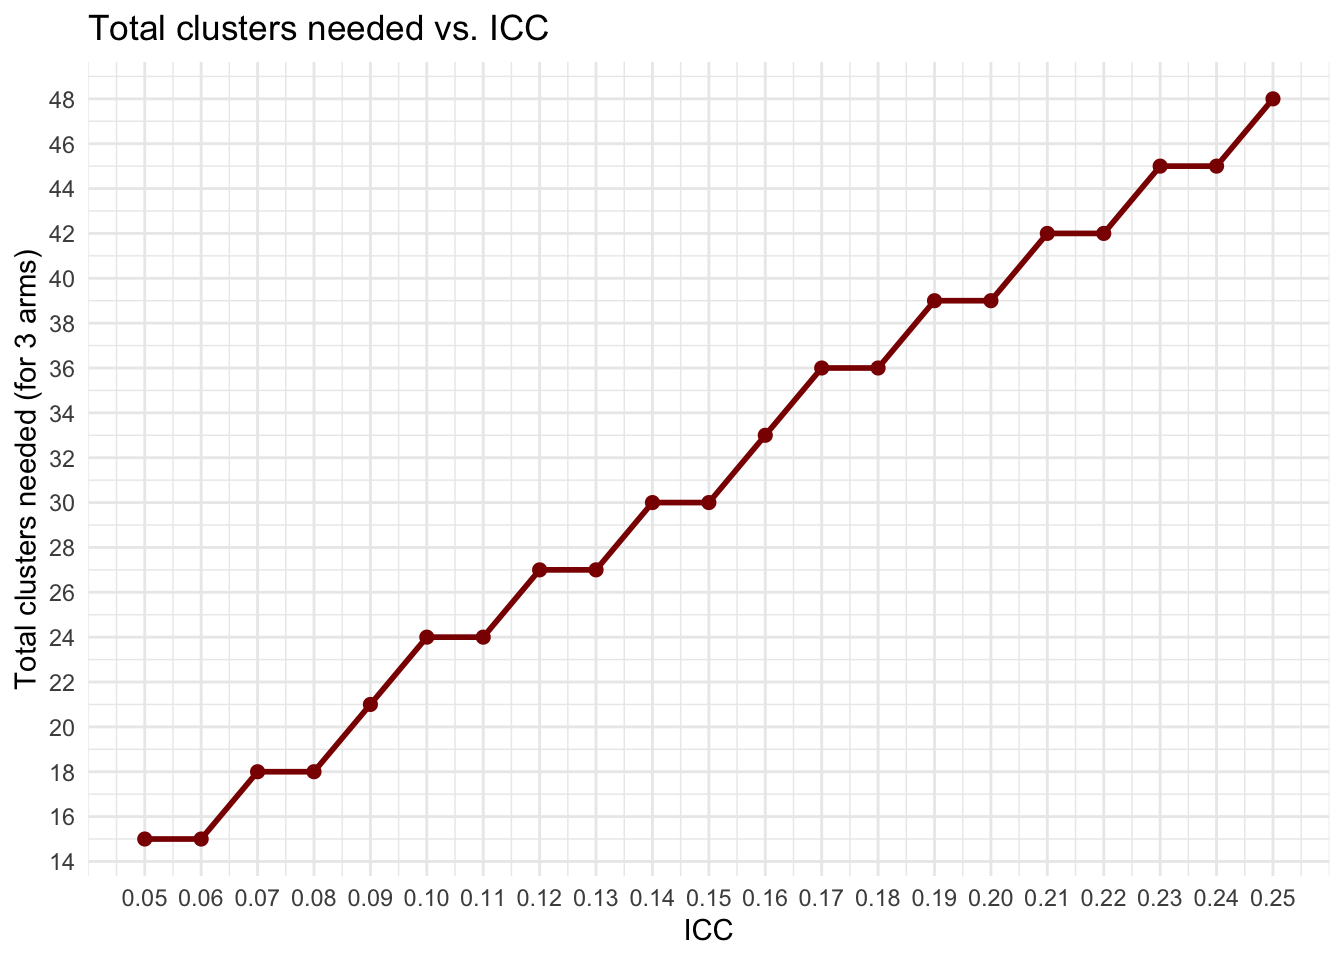
\includegraphics[keepaspectratio]{MOCA-DAWA_files/figure-pdf/unnamed-chunk-8-1.pdf}}

\begin{Shaded}
\begin{Highlighting}[]
\CommentTok{\# Plot number of individuals needed}
\FunctionTok{ggplot}\NormalTok{(results\_df, }\FunctionTok{aes}\NormalTok{(}\AttributeTok{x =}\NormalTok{ ICC, }\AttributeTok{y =}\NormalTok{ n\_individuals\_per\_arm }\SpecialCharTok{*} \DecValTok{3}\NormalTok{)) }\SpecialCharTok{+}
  \FunctionTok{geom\_line}\NormalTok{(}\AttributeTok{color =} \StringTok{"red"}\NormalTok{, }\AttributeTok{size =} \DecValTok{1}\NormalTok{) }\SpecialCharTok{+}
  \FunctionTok{geom\_point}\NormalTok{(}\AttributeTok{color =} \StringTok{"red"}\NormalTok{, }\AttributeTok{size =} \DecValTok{2}\NormalTok{) }\SpecialCharTok{+}
  \FunctionTok{labs}\NormalTok{(}
    \AttributeTok{title =} \StringTok{"Total individuals needed vs. ICC"}\NormalTok{,}
    \AttributeTok{x =} \StringTok{"ICC"}\NormalTok{,}
    \AttributeTok{y =} \StringTok{"Total individuals needed (for 3 arms)"}
\NormalTok{  ) }\SpecialCharTok{+}
  \FunctionTok{theme\_minimal}\NormalTok{() }\SpecialCharTok{+}
  \FunctionTok{scale\_x\_continuous}\NormalTok{(}\AttributeTok{breaks =} \FunctionTok{seq}\NormalTok{(}\FloatTok{0.05}\NormalTok{, }\FloatTok{0.25}\NormalTok{, }\AttributeTok{by =} \FloatTok{0.02}\NormalTok{)) }\SpecialCharTok{+}
  \FunctionTok{scale\_y\_continuous}\NormalTok{(}\AttributeTok{breaks =} \FunctionTok{seq}\NormalTok{(}\DecValTok{0}\NormalTok{, }\FunctionTok{max}\NormalTok{(results\_df}\SpecialCharTok{$}\NormalTok{n\_individuals\_per\_arm }\SpecialCharTok{*} \DecValTok{3}\NormalTok{), }\AttributeTok{by =} \DecValTok{100}\NormalTok{))}
\end{Highlighting}
\end{Shaded}

\pandocbounded{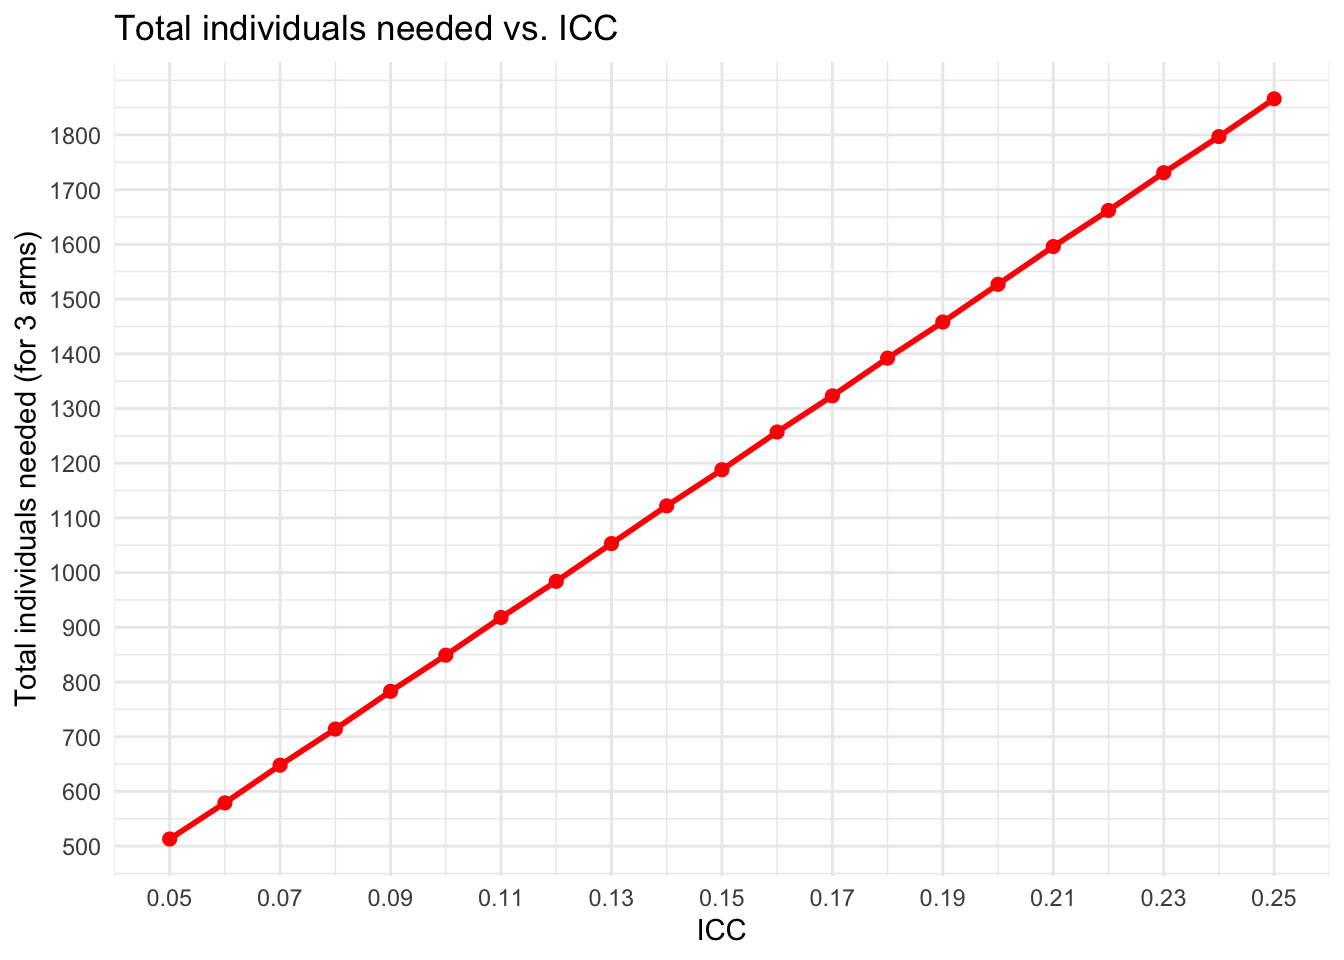
\includegraphics[keepaspectratio]{MOCA-DAWA_files/figure-pdf/unnamed-chunk-9-1.pdf}}

\paragraph{\texorpdfstring{\textbf{(2) Let's figure out the outcome
model}~}{(2) Let's figure out the outcome model~}}\label{lets-figure-out-the-outcome-model}

We have a binary outcome and plan to use a mixed-effects logistic model
to model the log-odds (logit) of success. We convert the linear
predictor into a probability using the inverse logit (logistic function)
and will draw from a Bernoulli distribution:

P(Y\_ij=1) = e\_nij/(1+e\_nij) , whereby nij = c\_j + β*rx\_j (the
linear predictor for individual i in cluster j)

\begin{itemize}
\item
  c\_j = the random cluster effect (cluster-specific deviation from the
  overall average)
\item
  β = the regression coefficient
\item
  rx\_j = the treatment status of cluster j
\end{itemize}

After fitting the logistic regression, the inverse logit function is
used to convert the log-odds (i.e., e\_nij) back into a probability.

\textbf{(3) Let's figure out the
ICC:}~ICC=textBetween−sitevariance/textTotalvariance, whereby the
between-site variance represents the clustering.

In logistic models, the ICC is usually fixed at:~pi2/3=3.29~for the
residual level (individual variation).

So, the between-site variance (sigma2\_c), i.e.~cluster-level noise, is
what we need, and is therefore derived as:

ICC=sigma2\_c/(sigma2\_c+(pi2/3))

(If there's additional within-site variation over time, i.e.~baseline
period, we include~sigma2\_cp, typically as a fraction of~sigma2\_c,
e.g., half the site-level variance -\textgreater{} for a later stage).




\end{document}
